\documentclass[11pt,a4paper]{moderncv}

% ModernCV themes
\moderncvstyle{banking}
\moderncvcolor{black}

% Adjust the page margins
\usepackage[top=1.5cm, bottom=1.3cm, left=1.3cm, right=1.3cm]{geometry}
\usepackage{tikz}
\usepackage{graphicx}


% Personal data
\name{}{Sahil Sanjay Rajpurkar}
\address{\faMapMarker*~M\"onsheim, Baden-W\"urttemberg, Germany}
\phone[mobile]{+49 17671678983}
\email{sahilrajpurkar1998@gmail.com}
\extrainfo{%
  \faLinkedin\ \href{https://www.linkedin.com/in/sahilrajpurkar}{LinkedIn} \quad 
  \faGithub\ \href{https://github.com/sahilrajpurkar}{GitHub} \quad 
  \faMedium\ \href{https://medium.com/@sahilrajpurkar}{Medium} \quad 
  \faRobot\ \href{https://sahilrajpurkar03.github.io}{Portfolio}%
}
\begin{document}

\makecvtitle
\pagestyle{empty}

\begin{tikzpicture}[remember picture,overlay]
  \node[anchor=north east, xshift=-1.3cm, yshift=-1.3cm] at (current page.north east)
    {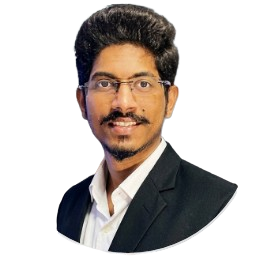
\includegraphics[width=2.8cm]{photo}};
\end{tikzpicture}

\vspace{-10mm}
% Education
\section{Education}
\cventry{Oct 2022 -- Feb 2025}{M.Sc. in Automation and Robotics}{Technical University of Dortmund}{Dortmund, Germany}{CGPA: 2.3}{%
  Major: Robotics%
}
\cventry{Aug 2016 -- Jul 2020}{B.Tech. in Electronics \& Telecommunication Engineering}{Mumbai University -- K.J. Somaiya College of Engineering}{Mumbai, India}{CGPA: 2.0}{%
  Major: Embedded Systems%
}

% Skills
\section{Skills}
\cvitem{Programming \& Tools}{Python, C++, Embedded C, MATLAB, Bash, Git, Docker, Linux}
\cvitem{Robotics \& Simulation}{ROS/ROS2, MoveIt, Gazebo, RViz, Isaac Sim/Lab, MuJoCo, DDS, WebSocket}
\cvitem{AI \& Data Processing}{OpenCV, TensorFlow, PyTorch, NumPy, Pandas, Matplotlib}
\cvitem{Embedded Systems}{STM32, ESP32, ARM, PCB Design (KiCad/Altium), RTOS, HIL, CI/CD Jenkins}
\cvitem{Sensors \& Hardware Integration}{LiDAR, Radar, IMU, Cameras, Sensor Fusion, Prototyping, Soldering}
\cvitem{Languages}{English (Business Fluent - C1), German (Intermediate - B1), Hindi, Marathi (Native)}

% Experience
\section{Experience}
\cventry{Apr 2026 -- Present}{Praktikant Humanoid Robotics: Development \& Validation}{Porsche Engineering}{M\"onsheim, Germany}{}{%
\begin{itemize}
    \item Developing localization, mapping, and navigation pipelines for wheeled mobile, quadruped, and humanoid robot platforms using ROS2, DDS, and WebSocket-based communication architectures.
    \item Simulating and validating multi-platform robot behavior in NVIDIA Isaac Sim and MuJoCo prior to real-world deployment.
    \end{itemize}
}

\cventry{Apr 2023 -- Jan 2026}{Research Assistant}{Communication Networks Institute, TU Dortmund}{Dortmund, Germany}{}{%
\begin{itemize}
    \item Developed a LiDAR-based 3D object detection pipeline for mobile robots using NVIDIA Isaac Sim, ROS2, and Python.
    \item Implemented LIO-SLAM with point cloud coloring from camera feed, and integrated with MMDetection for object detection.
    \item Built a dual-arm air hockey system using UFactory xArms with ROS2 MoveIt and tablet-based control.
    \item Conducted drone interference analysis with spectrum data collection on multiple UAVs using Aaronia Spectran V6.
    \item Assisted at Deutsches Rettungsrobotik-Zentrum (DRZ) rescue robotics demonstrations, integrating mmWave health sensors on Boston Dynamics Spot and Scout robots with wireless data streaming to the control station.
    \end{itemize}
}

\cventry{Jul 2020 -- Sep 2022}{Research Assistant}{Biomedical Engineering and Technology Innovation Centre (BETiC) | IIT Bombay}{Mumbai, India}{}{%
\begin{itemize}
    \item Led medical device projects including ventilators and portable oxygen generators with ISO 13485 compliance.
    \item Integrated medical-grade sensors with STM32 and ATMEL microcontrollers using UART, SPI, and I2C protocols.
    \item Implemented real-time control and diagnostic algorithms in Embedded C using RTOS, managed with Git and Jenkins for CI/CD.
    \item Conducted hardware-in-loop testing, prototype validation, and hospital demonstrations to ensure safety and performance.
    \end{itemize}
}



\section{Thesis}

\cventry{Aug 2024 -- Feb 2025}{at Lehrstuhl für Förder- und Lagerwesen (FLW), TU Dortmund}{Master Thesis: Radar-Based Object Detection for Logistics Entities \href{https://github.com/sahilrajpurkar03/Master-Thesis}{\faGithub}}{Dortmund, Germany}{}{%
\begin{itemize}
    \item Developed an ML-based detection pipeline using TI IWR6843ISK mmWave radar for logistics automation.
    \item Collected a custom indoor logistics dataset of forklifts, robots, and KLT's for model training.
    \item Trained 2D and 3D detection models using YOLOv7, Detectron2, and OpenPCDet (PV-RCNN) for logistic entities.
    \item Validated against Vicon motion capture system, achieving a mean centroid error of 0.4--0.5 m.
    \end{itemize}
}

\newpage
\cventry{Jul 2019 -- Apr 2020}{at Mercury Pneumatic Pvt. Ltd.}{Bachelor Thesis: Controlled Motion of a Pneumatic Quadruped Robot \href{https://github.com/sahilrajpurkar03/Bachelor-Thesis}{\faGithub}}{Mumbai, India}{}{%
\begin{itemize}
    \item Designed a pneumatic quadruped robot with two active degrees of freedom per leg.
    \item Implemented walking and pronking gaits using C++ algorithms on STM32F4, replicating mechanical model sequences.
    \item Integrated sensors and actuators on a custom PCB, including IMU, relays, and MOSFET circuits for balance monitoring.
    \item Evaluated robot stability, achieving a mean tilt error of ±10° during walking and pronking gaits with IMU feedback.
    \end{itemize}
}

% Projects
\section{Projects}
\cvitem{Robotic Arm Pick-and-Place Chatbot \href{https://github.com/sahilrajpurkar03/FrankaChatPicker}{\faGithub}}{Simulating pick-and-place tasks on a 6-axis robotic arm via chatbot commands using ROS2, Isaac Sim, MoveIt, and FastAPI. Integrated YOLOv8 OBB for object detection and LLM model via Ollama (Phi3) for natural language command interpretation.}
\cvitem{UR5 Object Alignment with Imitation Learning \href{https://github.com/sahilrajpurkar03/UR5-Object-Alignment}{\faGithub}}{Trained a UR5 robotic arm for precise object alignment in NVIDIA Isaac Sim using imitation learning and LeRobot framework with diffusion policy algorithms. Managed data collection, structured episodes, and comprehensive model evaluation in photorealistic simulations.}
\cvitem{Chat-bot for SI/PI/EMC \href{https://github.com/sahilrajpurkar03/pcb-sipiemc-chatbot}{\faGithub}}{AI-based RASA NLU chatbot assisting PCB designers with Signal Integrity, Power Integrity, and Electromagnetic Compatibility issues. Integrated LTSpice APIs for on-platform electrical design simulations and real-time optimization.}
\cvitem{Additional Projects}{Line-Following Robot with Color Detection (e-Yantra, IIT Bombay), Newborn Sleep Apnea Detector, Pneumatic pH Paper Punching Machine, Camera-based Fire Detection and Extinguishing System, Autonomous 3-wheel drive, Color-based Sorting Machine and more.}

% Publications
\vspace{1mm}
\section{Publications}

\cvitem{2021}{\textbf{\href{https://publications.waset.org/10012225/gaits-stability-analysis-for-a-pneumatic-quadruped-robot-using-reinforcement-learning}{Gaits Stability Analysis for a Pneumatic Quadruped Robot Using Reinforcement Learning}}}

%Competitions 
\vspace{1mm}
\section{Competitions}

\cventry{Aug 2025}{Simulated line-following task in NVIDIA Isaac Sim, winning €150 cash and \$500 NVIDIA Brev Credits.}{\textbf{LycheeAI Isaac Tournament - NVIDIA} | 1\textsuperscript{st} Place}{Online}{}{}

\cventry{May 2021}{Presented a prototype shoulder brace with IR sensors for vital sign monitoring.}{eMEDHA 2021 - IIT Bombay | Best Creativity Award}{Mumbai, India}{}{}

\cventry{Aug 2019}{Led a 30-member team, programmed autonomous robots, implemented NAV and line-following algorithms.}{RoboCon 2019 - IIT Delhi | 5\textsuperscript{th} Place \& MATLAB Competition Winner}{Delhi, India}{}{}

\cventry{Nov 2019}{Contributed to off-track safety by implementing a fire-redundant IoT system with a thermal camera.}{Eco-marathon 2019 - Shell India | 1\textsuperscript{st} Place \& Safety Award}{Bangalore, India}{}{}



%Volunteer
\vspace{3mm}
\section{Volunteer Experience}

\cventry{17\textsuperscript{th} -- 21\textsuperscript{st} Jul 2024}{Assisted participants in using the vSTING module to simulate network degradation effects.}{RoboCup 2024}{Eindhoven, Netherlands}{}{}

\cventry{Nov 2022 – May 2023}{Organized events for international students, ensuring an inclusive and memorable experience.}{DEGIS - German Association for International Students}{Bochum, Germany}{}{}

\cventry{2\textsuperscript{nd} – 24\textsuperscript{th} Oct 2021}{Mentored hackathon participants on problem definition, pitch feedback, and hardware planning.}{eMEDIC - Medical Device Innovation Camp}{Mumbai, India}{}{}

\cventry{13\textsuperscript{th} -- 15\textsuperscript{th} June 2018}{Taught robotics fundamentals, guided Arduino workshops, and mentored student teams.}{Workshop - Introduction to Arduino at KJ Somaiya College of Engineering}{Mumbai, India}{}{}

%Certifications 
\vspace{3mm}
\section{Certifications}
\cvitem{Online Courses}{Machine Learning (Coursera), Agile Development \& Scrum (IBM), Version Control with Git (Atlassian)}

\end{document}
